\documentclass[border=10pt]{standalone}

\usepackage{tikz}
\usepackage{tikzsymbols}
\usetikzlibrary{calc,patterns,shapes.geometric}

\def\centerarc[#1](#2)(#3:#4:#5){\draw[#1] ($(#2)+({#5*cos(#3)},{#5*sin(#3)})$) arc (#3:#4:#5);}

\begin{document}
	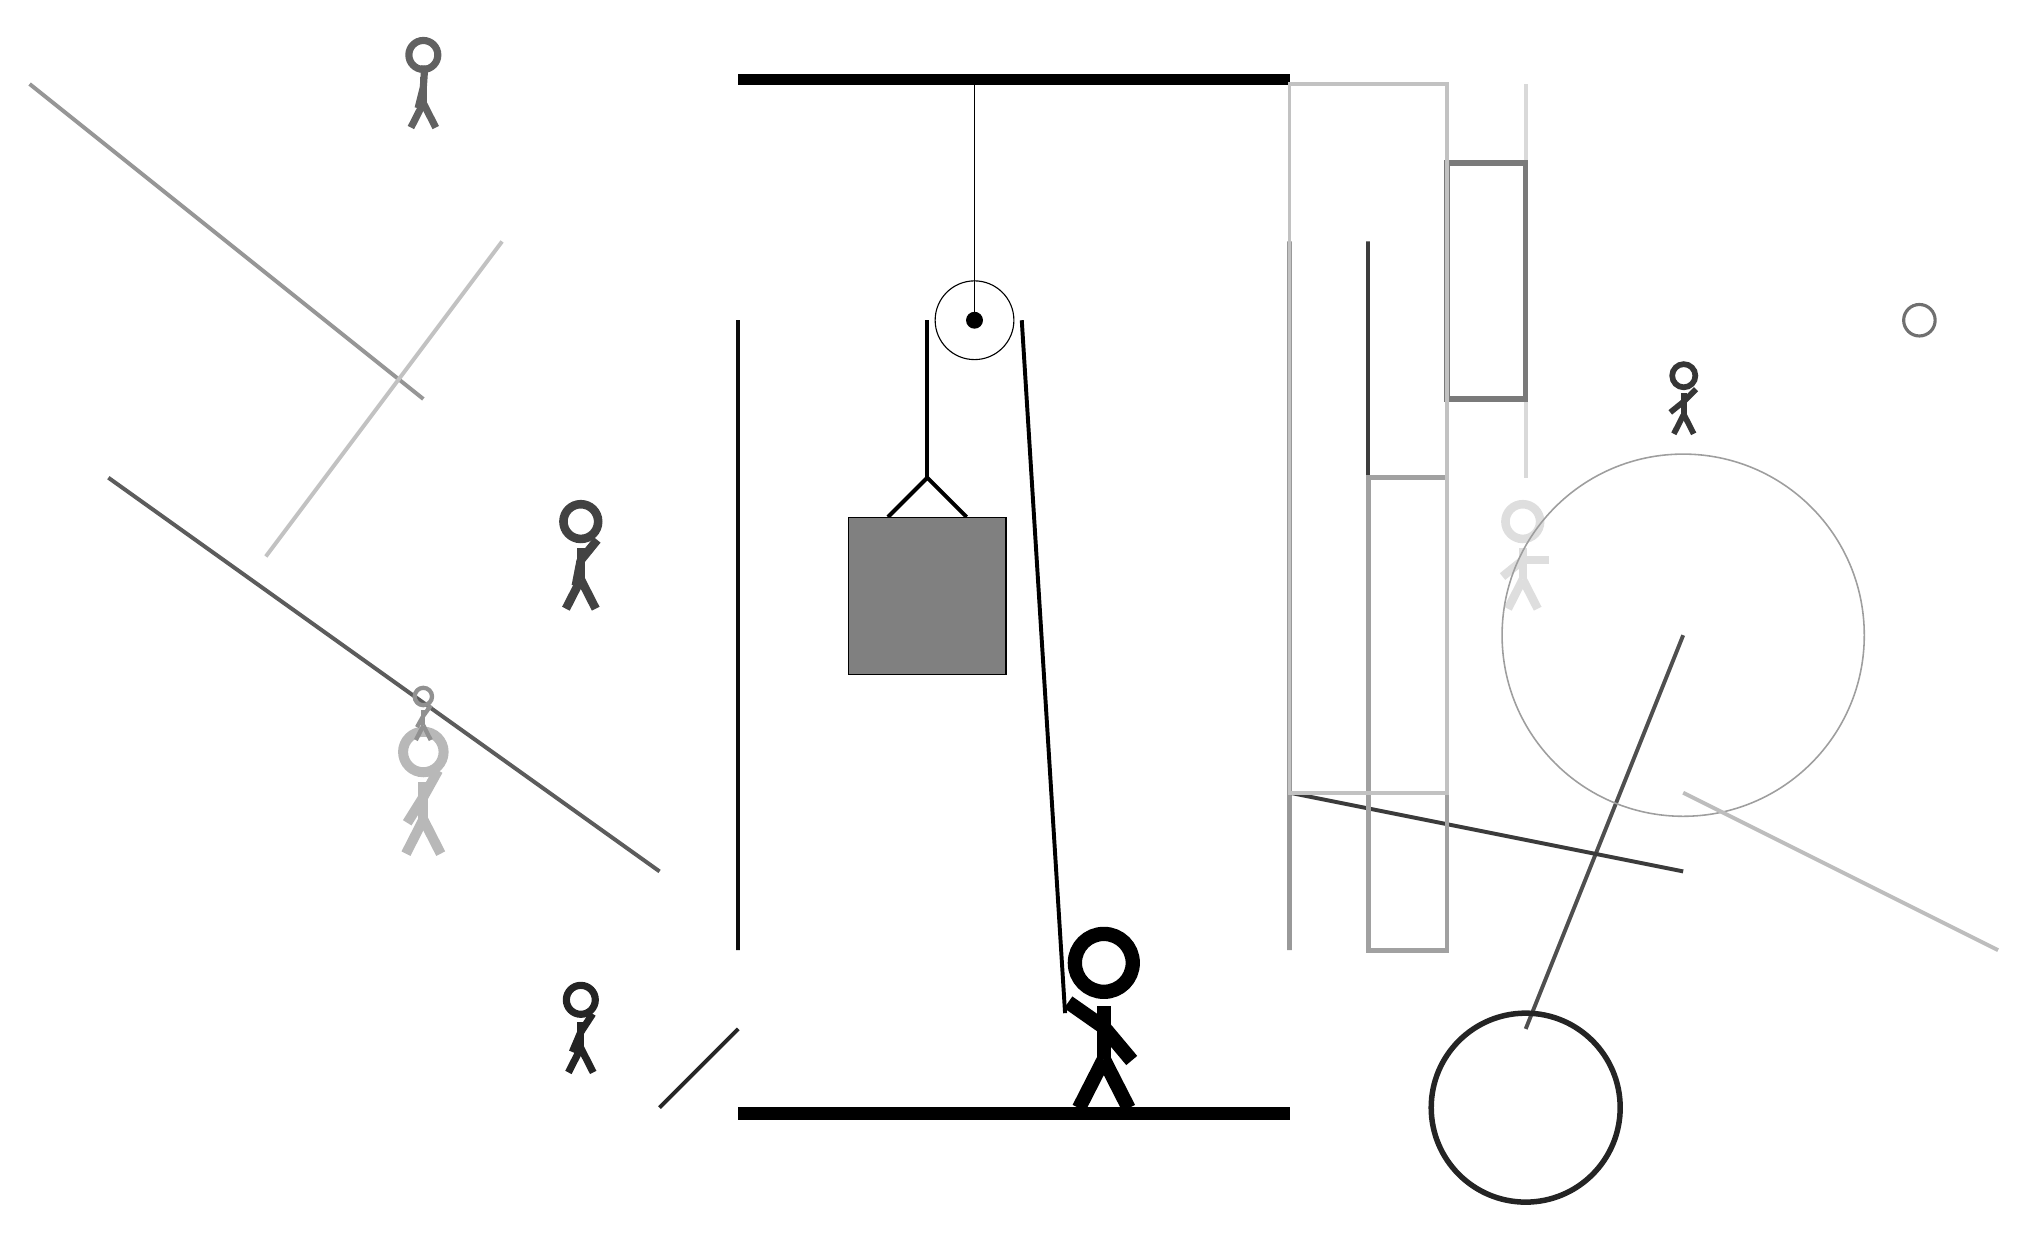
\begin{tikzpicture}
		%%%%% START %%%%%
		
		\draw[fill=black] (-2, 10) rectangle (5, 10.125);
		
		\draw (1, 7) circle (0.5);
		\draw[fill=black] (1, 7) circle (0.1);
		\draw (1, 10) -- (1, 7);
		
		\draw[line width=0.5mm] (-0.1, 4.5) -- (0.4, 5.0) -- (0.9, 4.5);
		\draw[fill=black!50] (-0.6, 4.5) rectangle (1.4, 2.5);
		
		\draw[line width=0.5mm] (0.4, 7) -- (0.4, 5.0);
		\centerarc[line width=0.5mm](1, 7)(0:180:0.6);
		\draw[line width=0.5mm](1.6, 7) -- (2.15, -1.8);
		
		\node at (2.6, -1.9) {\Strichmaxerl[10][-35][-50]};
		
		\draw[line width=0.5mm, color=black!64](-3, 0) -- (-10, 5);
		
		\draw[line width=0.6mm, color=black!40] (5, -1) rectangle (5, 8);
		\draw[line width=0.5mm, color=black!41](-6, 6) -- (-11, 10);
		\draw[line width=0.5mm, color=black!69](10, 3) -- (8, -2);
		
		\draw[line width=0.5mm, color=black!85](-3, -3) -- (-2, -2);
		\draw[line width=0.5mm, color=black!24](-5, 8) -- (-8, 4);
		\node[line width=0.4mm, color=black!13] at (8, 4) {\Strichmaxerl[6][39][0]};
		\draw[line width=0.2mm, color=black!76] (6, 7) rectangle (6, 3);
		\draw[line width=0.5mm, color=black!77](5, 1) -- (10, 0);
		
		\draw[line width=0.5mm, color=black!76] (6, 8) rectangle (6, 0);
		
		\node[line width=0.5mm, color=black!28] at (-6, 1) {\Strichmaxerl[7][58][61]};
		\draw [line width=0.4mm, color=black!56](13, 7) circle (0.2);
		\draw [line width=0.2mm, color=black!38](10, 3) circle (2.3);
		
		\draw[line width=0.6mm, color=black!37] (7, 5) rectangle (6, -1);
		\draw [line width=0.7mm, color=black!86](8, -3) circle (1.2);
		\node[line width=0.6mm, color=black!62] at (-6, 10) {\Strichmaxerl[5][76][86]};
		
		\node[line width=0.3mm, color=black!43] at (-6, 2) {\Strichmaxerl[3][61][54]};
		
		\draw[line width=0.5mm, color=black!15](8, 10) -- (8, 5);
		\draw[line width=0.7mm, color=black!52] (7, 9) rectangle (8, 6);
		
		\draw[line width=0.5mm, color=black!24] (7, 10) rectangle (5, 1);
		\draw[line width=0.5mm, color=black!95] (-2, 7) rectangle (-2, -1);
		
		\node[line width=0.5mm, color=black!79] at (10, 6) {\Strichmaxerl[4][39][45]};
		
		\draw[line width=0.5mm, color=black!26](10, 1) -- (14, -1);
		\node[line width=0.7mm, color=black!74] at (-4, 4) {\Strichmaxerl[6][79][51]};
		\node[line width=0.4mm, color=black!86] at (-4, -2) {\Strichmaxerl[5][67][57]};
		
		
		\draw[fill=black] (-2, -3) rectangle (5, -3.15);
		
		%%%%% END %%%%%
	\end{tikzpicture}
\end{document}